\documentclass[aspectratio=169,professionalfonts]{beamer}
\usetheme{Madrid}
\usecolortheme{default}
\usepackage[utf8]{inputenc}
\usepackage[T1]{fontenc}
\usepackage{lmodern}
\usepackage{amsmath}
\usepackage{booktabs}
\usepackage{tabularx}
\usepackage{array}
\usepackage{multicol}
\usepackage{tikz}
\usetikzlibrary{arrows.meta,positioning,fit,shapes.geometric,shapes.symbols,calc,matrix}
\usepackage{hyperref}

\definecolor{navy}{HTML}{123B5D}
\definecolor{teal}{HTML}{187D8D}
\definecolor{gold}{HTML}{D7A928}
\definecolor{soft}{HTML}{F4F7F9}
\definecolor{textgray}{HTML}{444444}
\setbeamercolor{structure}{fg=navy}
\setbeamercolor{title}{fg=white,bg=navy}
\setbeamercolor{frametitle}{fg=white,bg=navy}
\setbeamercolor{block title}{fg=white,bg=teal}
\setbeamercolor{block body}{bg=soft,fg=textgray}
\setbeamercolor{normal text}{fg=textgray,bg=white}
\setbeamercolor{item projected}{bg=teal,fg=white}
\setbeamerfont{title}{series=\bfseries,size=\Large}
\setbeamerfont{frametitle}{series=\bfseries,size=\large}
\setbeamertemplate{navigation symbols}{}
\setbeamertemplate{footline}[frame number]

\title{DAMA Chapter 4: Data Architecture}
\subtitle{Presentation overview with concepts, examples, and visual summaries}
\author{Prepared for Data Management Learning}
\date{Based on \emph{DAMA-DMBOK2}, Chapter 4}

\newcommand{\sourcefooter}{\vspace{0.4em}{\tiny Source: DAMA-DMBOK2, Chapter 4 (Data Architecture).}}

\begin{document}

\begin{frame}
  \titlepage
  \vspace{-0.5em}
  {\footnotesize This deck is based on the uploaded \emph{DAMA-DMBOK: Data Management Body of Knowledge, 2nd Edition}, especially Chapter 4 on Data Architecture.}
\end{frame}

\begin{frame}{Learning goals}
\begin{itemize}
    \item Understand what DAMA means by \textbf{data architecture} and why it matters.
    \item See how data architecture links \textbf{business strategy}, \textbf{data requirements}, and \textbf{technology execution}.
    \item Recognize core artifacts: \textbf{enterprise data models}, \textbf{subject area models}, and \textbf{data flows}.
    \item Identify practical activities, governance needs, and success factors for implementation.
\end{itemize}
\sourcefooter
\end{frame}

\begin{frame}{What is data architecture?}
\begin{columns}[T,totalwidth=\textwidth]
\column{0.58\textwidth}
\begin{block}{Core idea}
Data architecture is the \textbf{blueprint for managing data assets}. It describes how data is organized, defined, moved, controlled, and aligned with enterprise goals.
\end{block}
\begin{itemize}
    \item Covers artifacts, activities, and behaviors
    \item Works across multiple levels of abstraction
    \item Helps people understand data that is too large and complex to grasp directly
\end{itemize}
\column{0.42\textwidth}
\centering
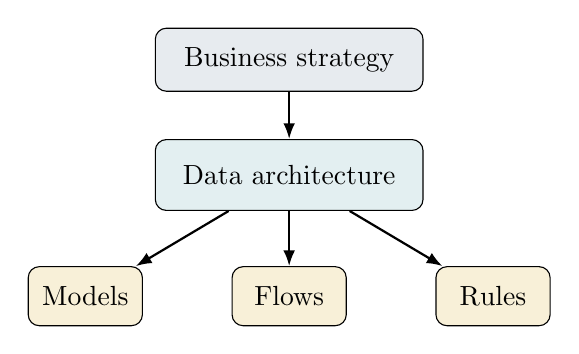
\begin{tikzpicture}[node distance=0.6cm]
\node[draw,rounded corners,fill=navy!10,minimum width=3.4cm,minimum height=0.8cm] (s) {Business strategy};
\node[draw,rounded corners,fill=teal!12,below=of s,minimum width=3.4cm,minimum height=0.9cm] (a) {Data architecture};
\node[draw,rounded corners,fill=gold!18,below left=0.7cm and 0.15cm of a,minimum width=1.45cm,minimum height=0.75cm] (m) {Models};
\node[draw,rounded corners,fill=gold!18,below=0.7cm of a,minimum width=1.45cm,minimum height=0.75cm] (f) {Flows};
\node[draw,rounded corners,fill=gold!18,below right=0.7cm and 0.15cm of a,minimum width=1.45cm,minimum height=0.75cm] (g) {Rules};
\draw[-{Latex[length=2mm]},thick] (s)--(a);
\draw[-{Latex[length=2mm]},thick] (a)--(m);
\draw[-{Latex[length=2mm]},thick] (a)--(f);
\draw[-{Latex[length=2mm]},thick] (a)--(g);
\end{tikzpicture}
\end{columns}
\sourcefooter
\end{frame}

\begin{frame}{Why organizations need it}
\begin{columns}[T,totalwidth=\textwidth]
\column{0.57\textwidth}
\begin{itemize}
    \item Bridges \textbf{business strategy} and \textbf{technology execution}
    \item Helps organizations evolve products, services, and data faster
    \item Makes sure processes consistently get the data they need
    \item Improves alignment between \textbf{business} and \textbf{IT}
    \item Supports agility, integration, and controlled change
\end{itemize}
\column{0.43\textwidth}
\begin{block}{Realistic examples}
\begin{itemize}
    \item Bank launching a new digital lending journey
    \item Hospital integrating patient, lab, and billing data
    \item Manufacturer shifting from selling products to \textit{pay-per-use} services
\end{itemize}
\end{block}
\end{columns}
\sourcefooter
\end{frame}

\begin{frame}{DAMA's 3-part view of data architecture}
\begin{columns}[T,totalwidth=\textwidth]
\column{0.48\textwidth}
\begin{block}{Three components}
\begin{enumerate}
    \item \textbf{Outcomes} -- models, definitions, data flows, roadmaps
    \item \textbf{Activities} -- forming, deploying, and maintaining architecture
    \item \textbf{Behavior} -- collaboration, mindset, and architectural discipline
\end{enumerate}
\end{block}
\column{0.52\textwidth}
\centering
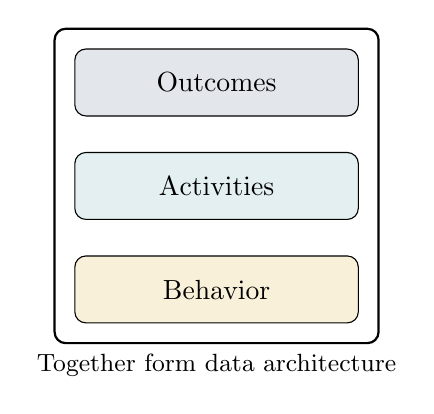
\begin{tikzpicture}[node distance=0.45cm]
\node[draw,rounded corners,fill=navy!12,minimum width=3.6cm,minimum height=0.85cm] (o) {Outcomes};
\node[draw,rounded corners,fill=teal!12,below=of o,minimum width=3.6cm,minimum height=0.85cm] (a) {Activities};
\node[draw,rounded corners,fill=gold!18,below=of a,minimum width=3.6cm,minimum height=0.85cm] (b) {Behavior};
\node[draw,rounded corners,thick,fit=(o)(a)(b),inner sep=0.25cm,label=below:{\small Together form data architecture}] {};
\end{tikzpicture}
\end{columns}
\sourcefooter
\end{frame}

\begin{frame}{Key outcomes and practice goals}
\begin{itemize}
    \item Define the \textbf{current state} of organizational data
    \item Provide a \textbf{standard business vocabulary} for data and components
    \item Align data architecture with \textbf{enterprise strategy} and \textbf{business architecture}
    \item Express \textbf{strategic data requirements} and high-level integrated designs
    \item Connect architecture work to the overall enterprise roadmap
\end{itemize}
\begin{block}{What good practice looks like}
Use architecture artifacts as master blueprints, influence projects and stakeholders, and establish the semantics of the enterprise through shared vocabulary.
\end{block}
\sourcefooter
\end{frame}

\begin{frame}{Architecture works across domains}
\small
\begin{tabularx}{\textwidth}{>{\bfseries}p{2.5cm}X X}
\toprule
Domain & Main focus & Example question \\
\midrule
Business architecture & How the enterprise creates value & Which capabilities and processes matter most? \\
Data architecture & How data should be organized and managed & What data do we need, and how should it fit together? \\
Applications architecture & Structure and function of applications & Which systems create or consume the data? \\
Technology architecture & Platforms, networks, and infrastructure & What technical environment hosts and protects the systems? \\
\bottomrule
\end{tabularx}

\vspace{0.6em}
\begin{block}{Takeaway}
Data architecture does not stand alone. It must work with business, application, and technology architecture.
\end{block}
\sourcefooter
\end{frame}

\begin{frame}{Enterprise architecture frameworks}
\begin{columns}[T,totalwidth=\textwidth]
\column{0.52\textwidth}
\begin{itemize}
    \item Frameworks help non-architects understand architecture relationships
    \item DAMA references common enterprise architecture frameworks
    \item The most visible example in the chapter is the \textbf{Zachman Framework}
    \item Zachman shows what models should exist from multiple stakeholder perspectives
\end{itemize}
\column{0.48\textwidth}
\centering
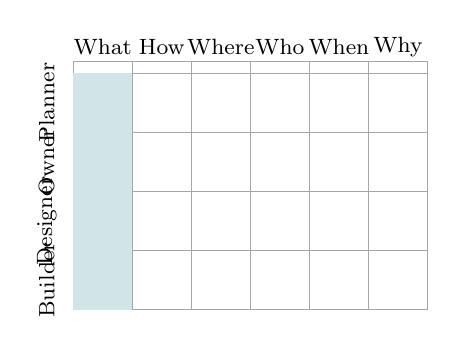
\begin{tikzpicture}[scale=0.75, font=\footnotesize]
\foreach \x in {0,...,5} {\draw[gray!70] (\x,0) rectangle +(1,4.2);} 
\foreach \y in {0,...,4} {\draw[gray!70] (0,\y) -- (6,\y);} 
\node at (0.5,4.45) {What};
\node at (1.5,4.45) {How};
\node at (2.5,4.45) {Where};
\node at (3.5,4.45) {Who};
\node at (4.5,4.45) {When};
\node at (5.5,4.45) {Why};
\tikzset{rowlabel/.style={rotate=90, font=\footnotesize}}
\node[rotate=90] at (-0.45,3.5) {\footnotesize Planner};

\node[rotate=90] at (-0.45,2.5) {\footnotesize Owner};

\node[rotate=90] at (-0.45,1.5) {\footnotesize Designer};

\node[rotate=90] at (-0.45,0.5) {\footnotesize Builder};
\fill[teal!20] (0,0) rectangle (1,4);
\end{tikzpicture}
\end{columns}
\sourcefooter
\end{frame}


\begin{frame}{Enterprise data model: the master blueprint}
\begin{columns}[T,totalwidth=\textwidth]
\column{0.55\textwidth}
\begin{itemize}
    \item The most detailed architecture design document is the \textbf{enterprise data model}
    \item It contains names, definitions, conceptual and logical entities, relationships, and business rules
    \item It is built across levels: conceptual \(\rightarrow\) subject area \(\rightarrow\) logical detail
    \item Physical models belong more directly to data modeling and design
\end{itemize}
\column{0.45\textwidth}
\centering
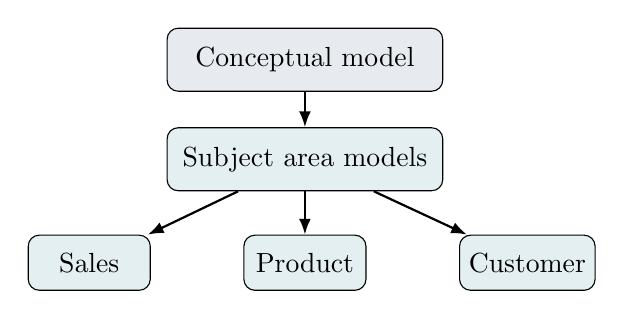
\begin{tikzpicture}[node distance=0.45cm]
\node[draw,rounded corners,fill=navy!10,minimum width=3.5cm,minimum height=0.8cm] (c) {Conceptual model};
\node[draw,rounded corners,fill=teal!12,below=of c,minimum width=3.5cm,minimum height=0.8cm] (s1) {Subject area models};
\node[draw,rounded corners,fill=teal!12,below left=0.55cm and 0.2cm of s1,minimum width=1.55cm,minimum height=0.7cm] (l1) {Sales};
\node[draw,rounded corners,fill=teal!12,below=0.55cm of s1,minimum width=1.55cm,minimum height=0.7cm] (l2) {Product};
\node[draw,rounded corners,fill=teal!12,below right=0.55cm and 0.2cm of s1,minimum width=1.55cm,minimum height=0.7cm] (l3) {Customer};
\draw[-{Latex[length=2mm]},thick] (c)--(s1);
\draw[-{Latex[length=2mm]},thick] (s1)--(l1);
\draw[-{Latex[length=2mm]},thick] (s1)--(l2);
\draw[-{Latex[length=2mm]},thick] (s1)--(l3);
\end{tikzpicture}
\end{columns}
\sourcefooter
\end{frame}

\begin{frame}{Subject area models make the enterprise understandable}
\begin{itemize}
    \item Each entity should live in one subject area, but can relate to entities in other areas
    \item Subject areas can be formed using normalization rules, ownership structures, value chains, or business capabilities
    \item DAMA notes that a \textbf{combined top-down and bottom-up approach} is often practical
\end{itemize}

\begin{block}{Example subject areas}
Customer, Product, Sales Order, Inventory, Supplier, Billing, Service, Claims.
\end{block}

\begin{block}{Teaching example}
In retail, \textit{Customer} belongs in one core subject area, but connects to orders, returns, support cases, and loyalty events across the enterprise.
\end{block}
\sourcefooter
\end{frame}

\begin{frame}{Data flow design and lineage}
\begin{columns}[T,totalwidth=\textwidth]
\column{0.56\textwidth}
\begin{itemize}
    \item Data flows show how data moves through processes and systems
    \item They reveal origin, storage, use, and transformation
    \item They can map relations between applications, data stores, networks, roles, and locations
    \item They support lineage analysis and better control of change
\end{itemize}
\column{0.44\textwidth}
\centering
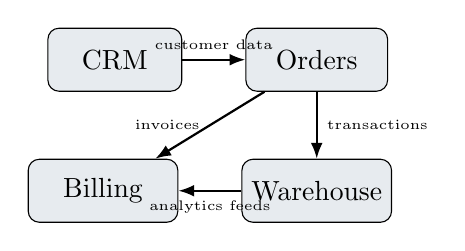
\begin{tikzpicture}[node distance=0.55cm]
\node[draw,rounded corners,fill=navy!10,minimum width=1.7cm,minimum height=0.8cm] (a) {CRM};
\node[draw,rounded corners,fill=navy!10,right=0.8cm of a,minimum width=1.8cm,minimum height=0.8cm] (b) {Orders};
\node[draw,rounded corners,fill=navy!10,below=0.85cm of b,minimum width=1.9cm,minimum height=0.8cm] (c) {Warehouse};
\node[draw,rounded corners,fill=navy!10,left=0.8cm of c,minimum width=1.9cm,minimum height=0.8cm] (d) {Billing};
\draw[-{Latex[length=2mm]},thick] (a)-- node[above,sloped]{\tiny customer data} (b);
\draw[-{Latex[length=2mm]},thick] (b)-- node[right]{\tiny transactions} (c);
\draw[-{Latex[length=2mm]},thick] (c)-- node[below,sloped]{\tiny analytics feeds} (d);
\draw[-{Latex[length=2mm]},thick] (b)-- node[left]{\tiny invoices} (d);
\end{tikzpicture}
\end{columns}
\sourcefooter
\end{frame}

\begin{frame}{Two useful ways to show data flow}
\begin{columns}[T,totalwidth=\textwidth]
\column{0.49\textwidth}
\begin{block}{1. Matrix view}
Best for showing which processes create, read, update, or depend on major entities.
\end{block}
\begin{tabular}{lcc}
\toprule
 & Customer & Order \\
\midrule
Sales & C/R & C/R \\
Billing & R & R/U \\
Support & R/U & R \\
\bottomrule
\end{tabular}

\column{0.49\textwidth}
\begin{block}{2. Diagram view}
Best for showing system-to-system movement and transformation of data.
\end{block}
\vspace{0.3em}
\centering
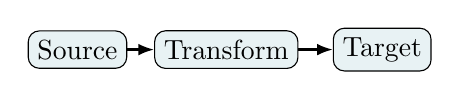
\begin{tikzpicture}[scale=0.9]
\node[draw,rounded corners,fill=teal!10] (x) at (0,0) {Source};
\node[draw,rounded corners,fill=teal!10] (y) at (2.1,0) {Transform};
\node[draw,rounded corners,fill=teal!10] (z) at (4.3,0) {Target};
\draw[-{Latex[length=2mm]},thick] (x)--(y);
\draw[-{Latex[length=2mm]},thick] (y)--(z);
\end{tikzpicture}
\end{columns}
\sourcefooter
\end{frame}

\begin{frame}{Interactive prompt: think like an architect}
\begin{block}{Mini discussion}
A university wants one trusted student record across admissions, exams, finance, and alumni systems.
\end{block}
\begin{enumerate}
    \item What should be the core subject areas?
    \item Where would the main data ownership conflicts appear?
    \item Which data flows would you document first?
\end{enumerate}
\vspace{0.5em}
\textbf{Possible starting answer:} Student, Course, Enrollment, Payment, Degree, Identity, and Communication.
\end{frame}

\begin{frame}{Activities: establish a data architecture practice}
\begin{itemize}
    \item Evaluate existing architecture specifications
    \item Develop a roadmap for target-state architecture
    \item Manage enterprise data requirements within projects
    \item Use architecture to reduce complexity and avoid uncontrolled system growth
\end{itemize}

\begin{block}{Why this matters}
Without active architecture practice, systems drift into copy-heavy, interface-heavy, low-trust environments --- what teams often call \textit{data spaghetti}.
\end{block}
\sourcefooter
\end{frame}

\begin{frame}{What architects actually do in practice}
\small
\begin{tabularx}{\textwidth}{>{\bfseries}p{3cm}X}
\toprule
Activity & Practical meaning \\
\midrule
Evaluate current state & Review models, interfaces, definitions, redundancies, and gaps \\
Roadmap target state & Decide the future blueprint, priorities, and transition path \\
Guide projects & Make sure new initiatives follow enterprise data requirements \\
Coordinate across domains & Align with business, application, and technology architects \\
\bottomrule
\end{tabularx}

\vspace{0.5em}
\begin{block}{Example}
When a telecom launches a self-care app, architects decide which customer, product, and billing data must stay authoritative and how the app should consume them.
\end{block}
\sourcefooter
\end{frame}

\begin{frame}{Integrating data architecture with enterprise architecture}
\begin{columns}[T,totalwidth=\textwidth]
\column{0.54\textwidth}
\begin{itemize}
    \item Data architecture must be integrated, not isolated
    \item Business capabilities drive data dependencies
    \item Application and technology choices must respect data requirements
    \item Architecture decisions should be visible in enterprise governance forums
\end{itemize}
\column{0.46\textwidth}
\centering
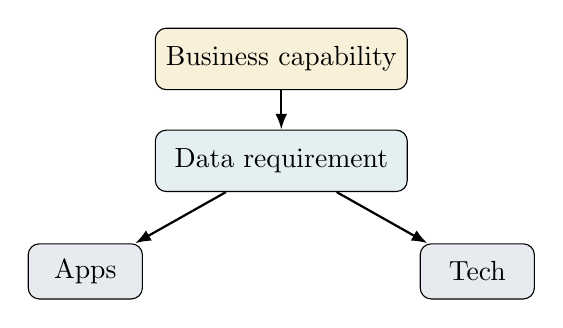
\begin{tikzpicture}[node distance=0.5cm]
\node[draw,rounded corners,fill=gold!18,minimum width=3.2cm,minimum height=0.78cm] (b) {Business capability};
\node[draw,rounded corners,fill=teal!12,below=of b,minimum width=3.2cm,minimum height=0.78cm] (d) {Data requirement};
\node[draw,rounded corners,fill=navy!10,below left=0.65cm and 0.15cm of d,minimum width=1.45cm,minimum height=0.7cm] (a) {Apps};
\node[draw,rounded corners,fill=navy!10,below right=0.65cm and 0.15cm of d,minimum width=1.45cm,minimum height=0.7cm] (t) {Tech};
\draw[-{Latex[length=2mm]},thick] (b)--(d);
\draw[-{Latex[length=2mm]},thick] (d)--(a);
\draw[-{Latex[length=2mm]},thick] (d)--(t);
\end{tikzpicture}
\end{columns}
\sourcefooter
\end{frame}

\begin{frame}{Tools and techniques from the chapter}
\begin{columns}[T,totalwidth=\textwidth]
\column{0.5\textwidth}
\begin{block}{Tools}
\begin{itemize}
    \item Data modeling tools
    \item Asset management software
    \item Graphical design applications
\end{itemize}
\end{block}
\column{0.5\textwidth}
\begin{block}{Techniques}
\begin{itemize}
    \item Lifecycle projections
    \item Diagramming clarity
\end{itemize}
\end{block}
\end{columns}

\vspace{0.5em}
\begin{block}{Simple message}
The tool does not create architecture quality by itself. Clear diagrams, consistent semantics, and disciplined lifecycle thinking do.
\end{block}
\sourcefooter
\end{frame}

\begin{frame}{Implementation guidelines and common risks}
\begin{itemize}
    \item DAMA explicitly highlights \textbf{readiness assessment} and \textbf{risk assessment}
    \item Implementation depends on organization and culture, not only design quality
    \item Architecture work needs communication, adoption, and behavior change
    \item Success requires balancing enterprise standards with local project realities
\end{itemize}

\begin{block}{Typical risks}
Poor buy-in, unclear ownership, weak standards adoption, over-complex diagrams, and projects bypassing enterprise architecture.
\end{block}
\sourcefooter
\end{frame}

\begin{frame}{Governance and metrics}
\begin{columns}[T,totalwidth=\textwidth]
\column{0.52\textwidth}
\begin{itemize}
    \item Data architecture needs governance to stay relevant and enforced
    \item Standards compliance is a major governance concern
    \item Metrics in the chapter include:
    \begin{itemize}
        \item architecture standards compliance rates
        \item trends in implementation
        \item business value metrics
    \end{itemize}
\end{itemize}
\column{0.48\textwidth}
\centering
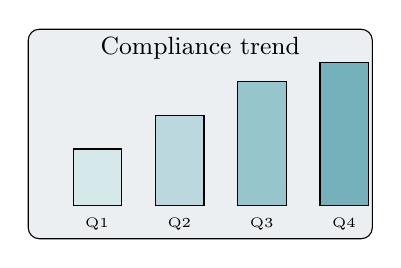
\begin{tikzpicture}[scale=0.95]
\draw[fill=navy!8,rounded corners] (0,0) rectangle (4.6,2.8);
\draw[fill=teal!18] (0.6,0.45) rectangle (1.25,1.2);
\draw[fill=teal!30] (1.7,0.45) rectangle (2.35,1.65);
\draw[fill=teal!45] (2.8,0.45) rectangle (3.45,2.1);
\draw[fill=teal!60] (3.9,0.45) rectangle (4.55,2.35);
\node[anchor=north] at (0.92,0.4) {\tiny Q1};
\node[anchor=north] at (2.02,0.4) {\tiny Q2};
\node[anchor=north] at (3.12,0.4) {\tiny Q3};
\node[anchor=north] at (4.22,0.4) {\tiny Q4};
\node at (2.3,2.55) {\small Compliance trend};
\end{tikzpicture}
\end{columns}
\sourcefooter
\end{frame}

\begin{frame}{Real-world style examples by section}
\small
\begin{tabularx}{\textwidth}{>{\bfseries}p{3cm}X}
\toprule
Section & Example \\
\midrule
Business drivers & Automotive firm adds connected-car services and now needs operational vehicle data as a managed asset \\
Enterprise data model & Insurer defines Party, Policy, Claim, Payment, and Product as shared enterprise concepts \\
Subject areas & University separates Student, Course, Enrollment, Finance, and Identity but keeps them related \\
Data flows & Hospital maps lab results from source system to EHR, billing, and analytics environments \\
Governance \& metrics & Retail group tracks compliance of new project schemas with enterprise customer definitions \\
\bottomrule
\end{tabularx}
\sourcefooter
\end{frame}

\begin{frame}{Interactive prompt: architecture trade-off}
\begin{block}{Scenario}
A company wants speed. Project teams want to copy customer data into every application because it is easier in the short term.
\end{block}
\begin{itemize}
    \item What short-term benefit are they chasing?
    \item What long-term data architecture risks appear?
    \item Where would you allow duplication, and where would you not?
\end{itemize}
\vspace{0.4em}
\textbf{Hint:} Use the language of trust, redundancy, lineage, integration cost, and ownership.
\end{frame}

\begin{frame}{Key takeaways}
\begin{enumerate}
    \item Data architecture is the enterprise \textbf{blueprint} for managing data assets.
    \item It connects \textbf{business strategy} to \textbf{data requirements} and then to \textbf{technology execution}.
    \item Its main artifacts are enterprise data models, subject area models, and data flow designs.
    \item It works only when integrated with broader enterprise architecture and governance.
    \item Good architecture reduces complexity, improves trust in data, and increases business agility.
\end{enumerate}
\sourcefooter
\end{frame}

\begin{frame}{Discussion / Q\&A}
\Large
\centering
Questions, reflections, or examples from your own organization?

\vspace{1em}
\normalsize
Possible prompts:
\begin{itemize}
    \item Where does your organization struggle most: models, flows, ownership, or standards?
    \item Which enterprise subject areas are hardest to define consistently?
    \item What architecture artifact would create the fastest business value for you?
\end{itemize}
\end{frame}

\begin{frame}[allowframebreaks]{Reference}
\footnotesize
Primary source used for the content structure and DAMA-aligned concepts in this deck:

DAMA International. \emph{DAMA-DMBOK: Data Management Body of Knowledge, Second Edition}. Technics Publications, 2017. Chapter 4: Data Architecture.

\vspace{0.7em}
Slides in this deck specifically reflect the chapter's definition of Data Architecture, its business drivers, architecture domains, enterprise data models, subject area models, data flows, activities, tools, techniques, implementation guidance, governance, and metrics.
\end{frame}

\end{document}
